\chapterstyle{texto}

% ----------------------------------------------------------
% Introdução (exemplo de capítulo sem numeração, mas presente no Sumário)
% ----------------------------------------------------------
\chapter{Introdução} \label{intro}
% ----------------------------------------------------------

\lipsum[2]


\chapter{Revisão Bibliográfica} \label{revisao}

Primeiro, é preciso preencher o arquivo Dados.tex para que suas informações sejam, devidamente passadas em todos os campos necessários no documento. Se sua banca tiver um terceiro avaliador favor alterar o arquivo em Pacotes/Face.sty e a linha em Dados.tex.

A seguir mostro os comandos principais a serem utilizados. Primeiramente, aqui está a citação com autor no final da frase \cite{nome_facil}. E também uma citação segundo \textcite{nome_facil} que aparece no meio da frase. Além disso é sempre possível também incluir uma citação longa que aparece com recuo conforme:

\begin{quote}
    \lipsum[3]\cite{nome_facil}
\end{quote}

Novos capítulos podem ser criados usando o comando \verb!\chapter!. Cada capítulo pode ser referenciado dinamicamente pelo \verb!\label! que acompanha ele. Assim se na frente a ordem do capítulo mudar a referencia se altera automaticamente no texto como vimos no capítulo \ref{revisao}. Novas seções podem ser iniciadas através do comando \verb!\section! . E também temos subsections e subsubsections de formas análogas.

Figuras podem ser inseridas no overleaf de maneira simples utilizando a interface gráfica. Aqui está uma figura num jeito mais ou menos pronto caso queira copiar. A figura também tem uma label que pode ser referenciada como na Figura \ref{fig:lei_potencias}. As figuras no latex são floats e possuem esses parâmetros h,b,t,p que influenciam seu posicionamento e dá pra saber mais \href{https://tex.stackexchange.com/questions/39017/how-to-influence-the-position-of-float-environments-like-figure-and-table-in-lat}{Nesse linkizinho do stackexchange de tex}. Que inclusive vai ser seu melhor amigo quando surgirem os primeiros problemas. 

\begin{figure}[h]
    \centering
    \caption{Simulação de uma lei de potência}
    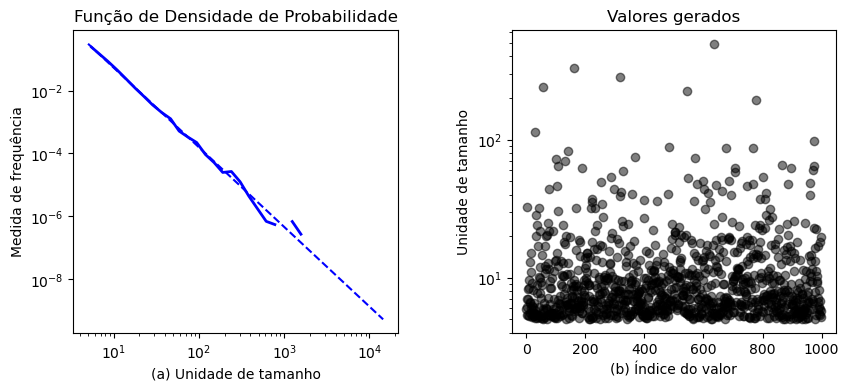
\includegraphics[width=1\linewidth]{Imagens/duas.png}
    \label{fig:lei_potencias}
    \captionsetup{font=footnotesize}
    \vspace*{-7mm}
    \caption*{Fonte: Elaboração Própria}
\end{figure}


Também temos equações alinhadas pra ficarem bem bonitinhas. Com novas labels pra gente referenciar. Como nas equações \eqref{matrix_minus}, \eqref{matrix_x} e \eqref{matrix_y}. E se quiser botar uma matemática na linha mesmo basta Digitar entre simbolozinhos de dólar $x=y-x$

\begin{align} 
M(x,y) & \rightarrow  M(x,y) - 4 \label{matrix_minus}\\ 
M(x\pm 1,y) &\rightarrow  M(x\pm 1,y) + 1 \label{matrix_x}\\
M(x,y \pm 1) &\rightarrow  M(x, y\pm 1) + 1 \label{matrix_y}
\end{align}

Por fim um outro comando fácil de mostrar é o de notas de rodapé. \footnote{Que colocam uma notinha de rodapé lá embaixo na página}

\chapter{Modelagem} \label{modelagem}

\lipsum[5]
\section{Descrição do Modelo} \label{descrição}

\lipsum[5]

\section{Desenvolvimento do Modelo} \label{desenv}

\lipsum[10]

\subsection{Exploração do modelo}

\lipsum[10]

% ---
% Conclusão
% ---
\chapter{Conclusão} \label{conclusao}

\lipsum[10]